\documentclass[french, 12pt, a4paper]{article}
\usepackage[utf8]{inputenc} 
\usepackage[T1]{fontenc}
\usepackage[a4paper,left=2cm,right=2cm,top=2cm,bottom=2cm]{geometry}
\usepackage{babel}
\usepackage[pdftex]{graphicx}
\usepackage{hyperref}
\usepackage{fancyhdr}
\usepackage{lastpage}
\usepackage{enumitem}
\usepackage{setspace}
\usepackage[font=small,labelfont=bf]{caption}
\usepackage{listings}
\usepackage{xcolor}
\usepackage{longtable}
\usepackage[justification=centering]{caption}
\usepackage{pdfpages}

\title{Rapport TER}
\author{Clément Lebouis, Soline Lecomte, Vincent Kowalski}
\date{January 2020}


\pagestyle{fancy}
\fancyhf{}
\lhead{Rapport de TER - Clément Lebouis, Soline Lecomte, Vincent Kowalski}
\rfoot{Page \thepage \hspace{1pt} sur \pageref{LastPage}}

\lstset{
language = java,
tabsize = 4, %% set tab space width
showstringspaces = false, %% prevent space marking in strings, string is defined as the text that is generally printed directly to the console
commentstyle = \color{green}, %% set comment color
keywordstyle = \color{blue}, %% set keyword color
stringstyle = \color{red}, %% set string color
rulecolor = \color{black}, %% set frame color to avoid being affected by text color
basicstyle = \small \ttfamily , %% set listing font and size
breaklines = true, %% enable line breaking
morecomment=[s][\color{gray}]{@}{\ },
}

\hypersetup{
    colorlinks,
    citecolor=black,
    filecolor=black,
    linkcolor=black,
    urlcolor=blue
}

\renewcommand{\familydefault}{\sfdefault}

\newcommand{\HRule}{\rule{\linewidth}{0.5mm}}
\newcommand{\myparagraph}[1]{\paragraph{#1}\mbox{}\\}

\lstset{
   captionpos=b
}

\pagenumbering{arabic}


\begin{document}

\addtocontents{toc}{\protect\setstretch{0.85}}

\begin{titlepage}
  \begin{center}

    
\includegraphics[scale=0.5]{Images/UnivNantes.png}~\\[2.5cm]
    \textsf{\huge - Rapport de TER - }\\[0.5cm]
    \textsf{\Large Réalisé par Clément Lebouis, Soline Lecomte et Vincent Kowalski}\\[0.3cm]
    \textsf{\large Master 1 ALMA}\\[0.5cm]
    \textsf{\Large De Janvier à Mai 2020}\\[2cm]
        

    \HRule \\[0.4cm]
    { \huge \bfseries Projet LeJos\\[0.4cm] }

    \HRule \\[1.5cm]
    
\includegraphics[scale=0.5]{Images/logoLS2N.jpg}
    \\[0.5cm]
    \textsf{\large Laboratoire des Sciences et du Numérique de Nantes, Équipe AeLoS}\\[0.2cm]
    \large\emph{Responsable : } M. Pascal Andre 
	\\[1.5cm]

  \end{center}
\end{titlepage}

\newpage
\tableofcontents
\newpage

\section{Introduction}

Au cours de notre Master informatique Architecture Logicielle (ALMA), nous avons eu l'occasion de travailler sur un projet de recherche dans le cadre des TER,
exercice visant à nous offrir l'opportunité de découvrir le travail et métier de chercheur.

Nous avons pour notre TER été accueillis par l'équipe AeLoS, l'une des équipes du Laboratoire des Sciences du Numérique de Nantes spécialisée dans la recherche de méthodes afin de garantir la correction des logiciels. Nous avons eu pour responsable M.Pascal André, enseignant-chercheur de l'équipe, et nous avons aussi été guidés et aidés par Mohammed Tebib, un ancien étudiant à l'Université de Nantes toujours en collaboration avec M.André.

Notre projet avait comme objectif le passage d'un modèle de programmation UML au code correspondant dans la continuité de plusieurs projets, effectués eux aussi dans le cadre de TER les années précédentes.
Afin d'éviter que le sujet ne soit trop large, il a été centré autour de la génération de code Java permettant le déplacement et le contrôle d'un petit véhicule motorisé.
\bigskip

Dans ce rapport, nous commencerons par parler des différents éléments constituant le projet global, de la façon dont nous les avons compris et essayé de les prendre en main. Puis nous rentrerons plus dans le détail des trois solutions principales qui ont été envisagées afin de permettre de représenter et de transiter au sein d'un graphe. Nous exposerons ensuite un rapport des différents frameworks trouvés, en rapport avec la solution que nous avons choisi d'explorer. Nous présenterons le framework qui a été choisi pour continuer le projet, puis nous continuerons avec la génération de code qui a été mise en place avec et sans l'utilisation de ce framework, avant de finir avec les possibilités mises à disposition mais n'ayant pas encore été exploitées.


\section{Prise en main}
    \subsection{Du modèle au code}

Au début de notre projet, nous avons commencé par tenter de prendre en main le sujet en lisant et en synthétisant les différentes informations utiles que nous pourrions trouver dans les documents fournis, notamment dans les dépôts git des autres projets. Voici ce que nous en avons retiré. 
\newline
\newline
Pour la mise en oeuvre de cette partie nous utilisons un robot Lego EV3 3 avec une application Android servant de télécommande. Deux alternatives se présentent alors  lorsque l'on souhaite générer du code à partir d'un modèle UML : le développement manuel ou la génération automatique de code.

\myparagraph{Le développement manuel}

Cette étape consistera premièrement en la modélisation du code à développer. Cette modélisation sera faite avec un diagramme de state machine selon la norme UML. Après la définition de ce modèle, le développement du code correspondant se fera manuellement, le code sera alors entier et fonctionnel.

\myparagraph{La génération automatique de code}

La génération automatique de code a pour objectif de retirer de la charge de travail au développeur en générant automatiquement la structure du code. 
Dans cette partie, qui représente notre sujet de projet, nous utilisons des éditeurs UML tels que StarUML, Papyrus, Visual Paradigm, etc. 
L'intérêt de passer par un éditeur est de trouver une manière générique et constante de représenter nos modèles, plutôt que de les développer manuellement en y ajoutant seulement ce qui nous semble nécessaire et à notre façon. Cependant, ces outils restent très limités et des problèmes liés à leur utilisation se feront remarquer plus tard lorsque nous souhaiterons générer des diagrammes de state machine plus élaborés.

De la manière la plus simple, la génération peut rester incomplète. Si, dans le diagramme de state machine, l'ensemble des fonctions nécessaires à l'exécution sont renseignées, le développeur n'aura plus par la suite qu'à remplir les dites fonctions afin de rendre le code fonctionnel.

Afin d'augmenter la responsabilité de la génération du code et de simplifier encore le travail du développeur, des contraintes OCL peuvent être ajoutées et ainsi décrire le fonctionnement des fonctions simples. Cette approche rajoutera un travail supplémentaire lors de la conception du modèle, mais surtout rajoutera des règles de conception du modèle qui dépasseront les limites de la norme UML.


\subsection{ATL}
Afin de permettre la prise en main d'ATL, nous avons demandé conseil à Mohammed Tebib, qui nous a guidé vers un tutoriel simple et expliquant bien chaque point : \url{https://wiki.eclipse.org/ATL/Tutorials_-_Create_a_simple_ATL_transformation}. Ce dernier nous a permis de mieux comprendre certains points.

L'ATL est un langage de transformation de modèle créé à Nantes par l'équipe de recherche AtlanMod (maintenant NaoMod) spécialisée dans le MDE (Model Driven Engineering). Son utilisation est possible grâce à l'installation d'un plug-in Eclipse. 

L'ATL permet, en partant d'un modèle source (dans notre cas un modèle UML), d'un ensemble de règles définies en ATL, et de deux métamodèles, de générer automatiquement un modèle cible. Les métamodèles correspondent à ce qui va permettre de générer les modèles. En effet, ces derniers définissent la structure à laquelle devra se conformer le modèle. Grâce à cela, nous allons définir des règles en ATL permettant de lier le métamodèle source avec le metamodèle cible, et le modèle cible sera ensuite généré automatiquement. Il nous a été nécessaire de visualiser les différentes étapes ainsi que les résultats pour bien en comprendre le fonctionnement. En voici donc un exemple, tiré du tutoriel fourni par Mohammed Tebib portant sur une transformation d'une structure de famille avec des membres à une structure de personnes avec un genre.
    
	\begin{center}
				\captionsetup{type=figure}
				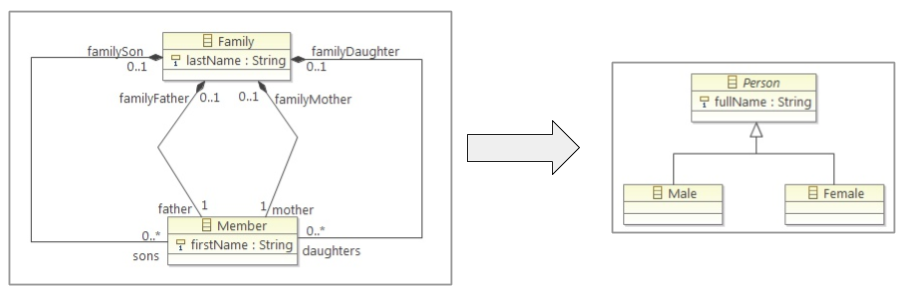
\includegraphics[scale=0.55]{Images/UML.png}
				\captionof{figure}{Diagramme UML du metamodèle source et du métamodèle cible.}
	\end{center}
    
    
	\begin{lstlisting}[caption={Un helper défini en ATL, permettant ensuite le définition des règles. Ici, le helper regarde si le membre de la famille est une fille ou non.}]
    helper context Families!Member def: isFemale(): Boolean =
      if not self.familyMother.oclIsUndefined() then
        true
	  else
        if not self.familyDaughter.oclIsUndefined() then
          true
        else
          false
        endif
      endif;
	\end{lstlisting}
	
	\begin{lstlisting}[caption={Une règle définie en ATL. Celle-ci détermine le genre du membre de la famille en utilisant le helper défini au dessus.}]
    rule Member2Female {
      from
        s: Families!Member (s.isFemale())
      to
        t: Persons!Female (
          fullName <- s.firstName + ' ' + s.familyName
        )
    }
	\end{lstlisting}
	
	
	\begin{lstlisting}[caption={Le modèle source défini en XML. Celui-ci a bien une structure de famille, et nous cherchons à changer cette structure pour obtenir une simple liste de personnes.}]
    <?xml version="1.0" encoding="ISO-8859-1"?>
    <xmi:XMI xmi:versi...... xmlns="Families">
    	<Family lastName="March">
    		<father firstName="Jim"/>
    		<mother firstName="Cindy"/>
    		<sons firstName="Brandon"/>
    		<daughters firstName="Brenda"/>
    	</Family>
    	<Family lastName="Sailor">
    		<father firstName="Peter"/>
    		<mother firstName="Jackie"/>
    		<sons firstName="David"/>
    		<sons firstName="Dylan"/>
    		<daughters firstName="Kelly"/>
    	</Family>
    </xmi:XMI>

	\end{lstlisting}

	\begin{lstlisting}[caption={Le modèle cible défini en XML, et généré automatiquement par Eclipse grâce aux métamodèles et aux règles définies précedement en ATL. Nous obtenons bien une structure de la forme liste de personnes.}]
    <?xml version="1.0" encoding="ISO-8859-1"?>
    <xmi:XMI xmi:versi....... xmlns="Persons">
    	<Male fullName="Jim March"/>
    	<Male fullName="Brandon March"/>
    	<Male fullName="Peter Sailor"/>
    	<Male fullName="David Sailor"/>
    	<Male fullName="Dylan Sailor"/>
    	<Female fullName="Cindy March"/>
    	<Female fullName="Brenda March"/>
    	<Female fullName="Jackie Sailor"/>
    	<Female fullName="Kelly Sailor"/>
    </xmi:XMI>

	\end{lstlisting}
    
Ce tutoriel nous a permis de découvrir le fonctionnement général d'ATL, par la mise en place de ses helpers, qui correspondent au méthodes dans du code Java par exemple, et qui seront appelés par les règles (rules), qui constituent des règles à appliquer pour le passage d'un modèle à un autre. De plus, nous avons pu commencer à ce point à découvrir la syntaxe bien particulière de l'ATL.

    
    \subsection{Chaine de transformations}
    Bien que nous nous soyons concentrés, lors de ce projet, sur la transformation d'un diagramme de state machine à du code, la finalité recherchée serait la mise en place d'une chaîne de transformation complète accompagnant le développement.
    
    Les diagrammes UML sont des approches génériques de la conception, indépendants de tout langage de programmation. C'est la raison pour laquelle il n'est pas possible de générer directement du code fonctionnel depuis des diagrammes UML. Mais des variantes, des versions plus spécifiques de ces diagrammes existent afin de se rapprocher d'un types de programmation particulier jusqu'à atteindre un niveau de quasi-équivalence avec un langage spécifique.
    
    Nous avons pu nous référer au livre :
    \textit{"Développement de logiciels avec UML 2 et OCL", de Pascal André et Alain Vailly, Chapitre 7 : Conception, de la transformation de modèles}. Dans ce dernier, la figure 233 (visible notamment page 308), met en évidence une hiérarchie de modèles, en soulignant la possibilité d'effectuer une transformation d'un modèle à un autre (de manière descendante ou ascendante) afin d'arriver à un langage spécifique. Dans le cadre de la programmation Java de ce projet, la hiérarchie à suivre serait ainsi de partir de la norme UML puis d'effectuer des transformations vers les modèles UML-PPO, puis UML-PPO-HS, et enfin UML-PPO-HS-NM avant de pouvoir envisager une transformation en code Java.
    
    Bien que des transformations soit envisageables afin de passer d'un modèle à un autre, si l'ensemble des informations nécessaires était présentes dès le départ, il n'y aurait pas de problèmes à passer directement de l'UML au Java. De fait, chaque diagramme apporte des possibilités et contraintes nouvelles. L'objectif de la chaîne de transformation serait ainsi de générer à partir de l'UML le maximum de la structure et des informations du modèle UML-PPO en ne laissant que peu de vides à compléter par les développeurs, puis reproduire cette mécanique en passant au modèle suivant jusqu'à arriver au code souhaité.
    
    
    \subsection{Le robot}
    Pour ce projet, un robot Lego Mindstorm EV3 a été mis à notre disposition.
    Malheureusement de nombreux problèmes ont été rencontrés durant les nombreuses tentatives de connection entre l'EV3 et l'ordinateur, principalement dues soit aux pilotes de windows ne permettant pas de manipuler ce genre d'appareils, soit aux périphériques n'en détectant pas la présence.
    
    À ce titre, la manière la plus simple qui a été trouvée afin d'effectuer cette connexion nécessite l'utilisation d'un adaptateur USB Wi-Fi. Une fois l'adaptateur branché à l'EV3, l'activation du Wi-Fi dans les paramètres de ce dernier permettra de se connecter aux réseaux Wi-Fi l'entourant. A partir de ce moment, un ordinateur présent sur le même réseau Wi-Fi pourra se connecter à l'EV3 afin de pouvoir lui envoyer les instructions à suivre.


\section{Automatisation des transitions}
    Le modèle principalement utilisé étant le diagramme de state machine, ce dernier représente donc l'exécution du code sous la forme d'un graphe constitué grossièrement d'états et de transitions permettant de passer d'un état à l'autre. La question qui s'est alors posée a été de savoir comment représenter ces états et comment transiter d'un état à l'autre avec le code. Pour répondre à cette question, trois approches principales se sont détachées.
    
    \subsection{Utilisation de variables d'état}
    La première possibilité était l'utilisation de variables d'état. Cette approche avait déjà été réalisée par le groupe de TER de l'année 2018, mais pas complètement aboutie.
    
    L'idée principale est de développer le comportement des différents états du state machine, et de les associer à une variable indiquant l'état dans lequel se trouve le graphe à l'instant courant de l'exécution. Lorsque cette variable change, on considère alors que l'on a changé d'état et l'on exécute le code correspondant à l'état en question.
    
    Cette méthode peut sembler la plus simple d'approche, mais un code constitué principalement d'un switch changeant l'exécution du code en fonction d'une variable peu vite trouver ses limites dans sa capacité à être maintenu par la suite. Qui plus est, avec une programmation objet, des alternative plus organisés peuvent être envisagées. Ce sujet ayant donc déjà été traité, il n'en sera pas question dans ce rapport.
    
    \subsection{Utilisation du design pattern State Machine}
    La seconde possibilité était l'utilisation d'un patron de conception. Cette approche quant à elle avait déjà été mise en place par Mohammed Tebib, sont travail nous a notamment été d'une grande aide dans la découverte et l'apprentissage des transformations ATL.
    
    L'idée est ici encore de créer dans le code un graphe exécutable correspondant au diagramme de state machine, mais cette fois ci avec une approche beaucoup plus orientée objet. Il serait possible d'imaginer, pour l'exemple, avoir des classes Graphe et Noeud mettant en place le fonctionnement de base de l'exécution du graphe. Puis afin de créer un noeud personnalisé, nous pourrions alors créer une nouvelle classe, héritant de la classe Noeud principale, dans laquelle nous définirons les différentes spécificités du noeud en question.
    
    L'inconvénient apparaissant avec l'approche objet est la nécessité de créer plusieurs classes héritées d'un objet principal afin d'en décrire les spécificités. L'accumulation de différentes classes peut alors vite se retrouver pénible à maintenir, notamment sur des projets de taille conséquente.
    
    \subsection{Utilisation d'un framework}
    L'utilisation d'un framework est une approche complémentaire à celle des design patterns. En effet, dans cette dernière, le code à générer se distingue en deux parties principales, d'un coté toute la partie fonctionnelle qui permettra de créer un graphe et de l'exécuter. Et deuxièmement la partie descriptive, où à partir du diagramme de state machine nous allons créer des instances de ce graphe et de ses composants, instances dans lesquelles seront décrites les spécificités correspondant à un diagramme de state machine particulier pour un problème donné.
    
    Ce qu'il en ressort est qu'une partie du code est générale et inchangée entre les générations alors que l'autre partie s'adaptera et sera différente pour chaque diagramme de state machine qui sera donné en entrée. Hors, dans l'approche des design patterns, la transformation ATL est chargée de générer ces deux parties à chaque exécution et sera donc contrainte de regénérer à chaque fois la partie fonctionnelle.
    
    L'objectif de l'approche framework est d'alléger la charge de la génération ATL par l'utilisation d'un framework qui contiendra l'entièreté de la partie fonctionnelle. L'ATL n'aura donc par la suite que la partie descriptive à générer en créant les dépendances avec le diagramme (la partie fonctionnelle étant générée sans dépendance) et ce en appelant les classes et fonctionnalités mises à disposition par le framework.
    
    Dans cette approche, la question à été par la suite de savoir s'il serait plus judicieux de choisir un framework offrant déjà ces fonctionnalités, ou bien de créer notre propre framework, soit à partir de rien, soit en se basant sur un framework déjà existant mais incomplet. Par exemple un framework permettant de mettre en place un graphe exécutable mais n'étant pas au normes UML, ou bien à l'inverse un framework offrant la création d'un diagramme de state machine, mais ou la notion d'exécution est absentée.
    
    Nous avons opté pour cette méthode pour notre projet, car elle n'avait pas encore été exploitée, et semblait offrir des pistes très intéressantes pour notre génération automatique de code.
    


\section{Recherche de frameworks}
Ayant sélectionné la méthode que nous allions employer, il nous a fallu commencer à chercher des frameworks qui pourraient s'appliquer dans notre cas. Un partie de l'équipe s'est donc attelée à cette tâche, pendant que l'autre exploitait le dépôt git de Mohammed Tebib et essayait de s'approprier ce nouveau langage. 

    \subsection{UML Statechart Framework for Java}
    UML Statechart a été le premier framework que nous avons analysé afin de savoir si il irait avec nos futures expérimentations. Il nous a été proposé par M. André afin de guider notre recherche dans le vaste milieu des frameworks.
    
        \subsubsection{Principe}
        Comme tout les frameworks qui seront listé plus bas, UML Statechart a pour but de coller au maximum au fonctionnement des diagrammes "Statechart" et de permettre leurs écriture en code le plus facilement et rapidement possible. Pour cela, plusieurs étapes nous sont données par le créateur afin d'effectuer cette tache.
        
        \paragraph{Création des Évènements :}
        Il nous faut créer les classes pour chaque évènement (Event) utilisé dans le diagramme en les faisant hériter de la classe Event qui gère ce genre de choses dans ce framework. Ils seront utilisé dans la quatrième et dernière étape pour le fonctionnement de notre diagramme.
        
        \begin{lstlisting}
//Exemple d'evenements
public class anEvent extends Event {
    public anEvent() {
        super("anEvent");
    }
}
        \end{lstlisting}
        
        \paragraph{Création des Actions :}
        Maintenant que nos évènements sont créés il faut maintenant mettre en place les actions qui seront exécutées une fois dans un état, par exemple un print, ou l'augmentation / réduction d'une valeur. Deux types d'actions existent, les actions a l'entrée et celles a la sortie d'un état.
        
        \paragraph{Création des Guards :}
        La mise en place du Guard est une étape importante car elle nous permet l'utilisation de structure conditionnelle (If/Else). Nous pouvons voir le Guard comme la condition a vérifier pour décider dans quel état nous nous dirigerons.
        
        \begin{lstlisting}
//Exemple de Guard
//Cet exemple provient du GitHub du framework
public class ValueEquals extends Guard {
  private int value;

  public ValueEquals(int value) {
   this.value = value;
  }

  public boolean check(Metadata data, Parameter parameter) {
    return data.value == value;
  }
}
        \end{lstlisting}
        
        \paragraph{Création des États :}
        Nous devons maintenant, selon le créateur, créer la variable contenant l'objet Statechart qui est notre diagramme, ainsi que ses états initiaux et finaux principaux. Une fois ceci fait, nous devons créer chaque état et sous-état de manière a créer toutes les variables du diagrammes sans pour autant créer les transitions. Chaque état dispose ou non d'une action a effectuer en entrée et sortie de celui-ci.
        
        \paragraph{Création du diagramme Statechart :}
        Une fois que tout est en place, évènements, actions, guard,  états, nous effectuons la mise en place de toutes les transitions du diagramme. La création de transitions peut se faire avec cinq paramètres différents dont deux obligatoire: 
        \begin{lstlisting}
//Ces exemples proviennent du GitHub du framework
//Exemple d'instanciation du diagramme
Statechart chart = new Statechart();

//Definition de l'etat initial
PseudoState state_start = new PseudoState("start", chart, PseudoState.pseudostate_start);


//Definition de l'etat final
FinalState state_final = new FinalState("final", chart);
        \end{lstlisting}
        
        \begin{lstlisting}
//Exemples de transitions
new Transition(stateA, stateB);
new Transition(stateB, stateA, new TimeoutEvent(1000), new Print("Timeout"));
new Transition(stateB, stateC, new someEvent());
        \end{lstlisting}
        
        \subsubsection{Avantages et inconvénients}
        Le principal avantage de ce framework est sa rapidité d'implémentation ainsi que son désir de coller au maximum a la sémantique UML afin de permettre aux utilisateurs une plus grande facilité d'utilisation de celui-ci. A coté de cela, le principal inconvénient de ce framework serait le fait que le framework met en place la version 1.5 d'UML alors que nous sommes actuellement en version 2.4 .
    
    \subsection{Squirrel}
    Squirrel fut le framework le plus facile à trouver une fois que nous savions comment chercher. Il a une approche bien particulière tout en voulant coller a l'UML. C'est ce qui a fait que nous l'avons rajouté dans cette liste.
    
        \subsubsection{Principe}
        Squirrel a pour principe de représenter en code un diagramme de Statemachine pour l'exécuter.
        
            \paragraph{Construction des Évenements : }
            Les évènements ont une construction très simple avec ce framework, il suffit simplement d'écrire une énumération de la classe FSMEvent. Une fois ceci fait, ils seront utilisés a la fin pour la définition des transitions.
            
            \begin{lstlisting}
//Exemple d'evenements
enum FSMEvent {
    ToA, ToB, ToC, ToD
}
            \end{lstlisting}
            
            \paragraph{Construction du Statemachine : }
            Afin de construire le Statemachine, nous devons créer notre propre classe qui elle-même hérite d'un certain type de classe Statemachine fourni par Squirrel. La manière de créer un tel diagramme permet d'enchaîner avec la méthode de création des actions.
            
            \paragraph{Construction des Actions : }
            Pour chaque action dans le diagramme, nous allons créer une fonction prenant plusieurs paramètres.  Ceux-ci sont l'état de départ et d'arrivée, l'évènement qui permet l'action, ainsi que le contexte de celle-ci.
            
            \begin{lstlisting}
//Exemple d'action
public void fromAToB(MyState A, MyState B, FSMEvent event, Context context) {}
            \end{lstlisting}
            
            \paragraph{Construction des Transitions : }
            Les transitions sont construites de la manière suivante : nous allons, pour chaque transition, utiliser le builder de Statemachine de la façon suivante : 
            
            \begin{lstlisting}
//Exemple de transition
builder.externalTransition().from("A").to("B").on(FSMEvent.ToB).callMethod("fromAToB");
            \end{lstlisting}
            
            Nous choisissons l'état d'origine et d'arrivée, l'évènement censé appeler cette transition, ainsi que l'action à effectuer via la méthode "callMethod".
            
            
        \subsubsection{Avantages et inconvénients}
        Le principal avantage de Squirrel est la définition de ces objets qui semble assez intuitive à utiliser au premier abord. A coté de cela, le projet a une taille conséquente et l'utilisation des annotations, pour renseigner notamment les transitions, laisse penser qu'une tentative d'implémentation de framework héritant de ces classes pourrait s'avérer fastidieux.

    \subsection{JState}
    JState est un framework qui nous intéressait autant par sa simplicité de compréhension que sa facilité de mise en place en terme de programmation. Comme les autres frameworks, il essaye de mimer le fonctionnement des diagrammes Statemachine mais de manière plus simple et accessible.
    
        \subsubsection{Mise en place}
            \paragraph{Construction des états : }
            La mise en place des états se fait via la classe State fournie par JState. Contrairement à d'autres frameworks, nous n'avons pas à instancier de variables ou créer de classes pour les états, il nous suffit simplement de créer une énumération d'objet State, puis de s'en servir dans la mise en place des transitions.
            
            \begin{lstlisting}
//Exemple de declaration d'etats
enum State {
    Start, Stop, Shutdown, A, B, C
}
            \end{lstlisting}
            
            \paragraph{Construction du diagramme : }
            La mise en place du Statemachine se fait via la structure de données EnumStateMachine. Celle-ci nous permet de créer le diagramme de deux manières différentes, soit en lui donnant l'état initial en paramètre, soit en ne le précisant pas et donc en l'ajoutant plus tard.
            
            \begin{lstlisting}
//Instanciation du diagramme avec l'etat initial dans le constructeur
EnumStateMachine<State> stateMachine = new EnumStateMachine<>(State.Start);
            \end{lstlisting}
            
            \begin{lstlisting}
//Instanciation du diagramme sans l'etat iniatial dans le constructeur
EnumStateMachine<State> stateMachine = new EnumStateMachine<>();
stateMachine.setInitialState(State.Start);
            \end{lstlisting}
            
            \paragraph{Construction des Transitions \& Actions: }
            La mise en place des transitions se fait directement à la suite de l'instanciation du diagramme via la fonction addTransitions(). Comme l'indique le nom de la méthode, nous pouvons instancier plusieurs transitions en un seul appel. La création des transactions fonctionne aussi en parallèle avec la création des actions, ce qui nous donne trois grandes méthodes pour appliquer le addTransactions().
            
            \begin{lstlisting}
//Methode 1 : Transition simple entre deux etats
stateMachine.addTransitions(State.Start, State.A);
            \end{lstlisting}
            
            \begin{lstlisting}
//Methode 2 : Transition simple entre deux etats avec une actions
TransitionHandler<State> action = new TransitionHandler<>() {
    public void onTransition(State from, State to) {
        
    }
};
stateMachine.addTransitions(action, State.A, State.B);
            \end{lstlisting}
            
            \begin{lstlisting}
//Methode 3 : Transitions successive d'etats
stateMachine.addTransitions(State.Start, State.A, State.B);
            \end{lstlisting}
            
        \subsubsection{Avantages et inconvénients}
        Le grand avantage de ce framework est sa simplicité de mise en place et de compréhension, malheureusement en l'étudiant nous avons remarqué qu'il n'essayait pas vraiment de coller à un fonctionnement détaillé d'un Statemachine, mais plus d'être similaire à un graphe normal avec des transitions.

    \subsection{Comparaisons et choix du framework}
    Maintenant que nous avons listé et étudié le fonctionnement de chaque framework nous pouvons les comparer entre eux afin de décider lequel sera celui qui sera utilisé pour être la cible de la génération du code.
    
    Afin de faire une comparaison correcte, nous avons séparé en deux points majeurs chaque framework:
    \begin{itemize}
        \item Correspondance avec UML
        \item Facilité d'implementation du code
    \end{itemize}
    
        \subsubsection{Correspondance avec UML}
        Bien que chaque framework permette la mise en place d'un graphe, JState ne semble pas correspondre aux contraintes d'un diagramme UML de state machine. 
        
        Squirrel dans son cas parait prendre une logique et un visuel proche du diagramme de state machine mais ne semble affirmer nulle part la correspondance directe entre les deux, il y a donc d'éventuels ajustements à prévoir, ou tout du moins une vérification du respect de ces propriétés. 
        
        UML Statechart for Java a quant à lui mis en place un diagramme de state machine correspondant à la version UML 1.5 . Cette dernière peut paraître vielle, étant à ce jour en version 2.4, mais il est alors envisageable de travailler sur une base sûre, en prévision d'amélioration et de mise à jour future.
        
        \subsubsection{Facilité d'implémentation du code}
        Dû au fait qu'il n'existe quasiment aucun framework proposant un diagramme de state machine à jour et exécutable, il était évident qu'en définitive il y aurait des modifications à apporter au framework choisi, la question était donc de trouver un framework qui permettrait de facilement l'adapter à nos besoins, et qui permettrait également une implémentation assez simple et envisageable dans le contexte d'une génération avec ATL.
        
        Squirrel et UML Statechart for Java proposent tous les deux une notion de graphe exécutable. Squirrel est par contre un projet bien plus gros que UML Statechart for Java, et certaines notions comme l'utilisation d'annotation pour déclarer les transitions d'un état à un autre rend le tout assez difficile à prendre en main, et complexifie beaucoup la nature des objets constituant le projet, difficile donc d'entrevoir comment en hériter en vue d'ajout de fonctionnalités futures.
        
        UML Statechart for Java a pour sa part un nombre de classes plutôt réduit et la documentation mise à disposition permet rapidement de mettre en place un graphe simple que l'on peut complexifier par la suite. L'approche contre intuitive qu'il met en place, en ne proposant pas de classe noeud mais en centrant ses classes sur les transitions entre ces noeuds, a été surprenante, mais peut à terme se montrer intéressante pour l'organisation du projet. De fait un noeud dans un graphe est unique, mais une fonction peut être réutilisée par plusieurs noeuds avec des paramètres différents.

    \bigskip

    Une fois nos comparaisons effectuées, nous avons décidé d'utiliser UML-Statechart for Java de part la garanti de la mise en place d'un UML de base sûre, ainsi que d'une facilité de prise en main, étant un grand atout au vu du peu de temps nous restant à travailler sur le projet.

\section{Génération de code}
Afin de permettre la génération du code et étant très peu familiers avec ATL, nous avons décidé de suivre un procédé simple : 
    \begin{itemize}
        \item Créer un diagramme d'état-transition (StateMachine) s'appliquant à notre robot
        \item Écrire à la main le code que nous pensions lui être le mieux associé en utilisant le framework que nous avons choisi
        \item Programmer ensuite l'ATL qui prendrait le diagramme en entrée et qui devrait produire le code attendu, en généralisant au maximum afin que tout fonctionne avec un autre diagramme ayant la même structure
    \end{itemize}
    
    \subsection{Génération sans framework défini précisément}
    
    \subsubsection{Création du diagramme}
    Notre premier diagramme généré a été légèrement intuitif, car nous avons simplement créé un diagramme qui paraissait selon nous fonctionner avec notre robot. En effet, au moment de la création de ce diagramme, nous n'avions pas encore défini de framework à utiliser, et donc nous n'avions pas de structure particulière à suivre. 
    Nous avons donc défini dans notre diagramme un état par état que pouvait prendre le robot : arrêté, en train d'accélérer, en train d'avancer, en train de reculer, en train de ralentir ou éteint. 
    Ensuite, nous avons mis en place les transitions, qui correspondaient aux fonctions appelées pour passer d'un état à un autre. 
    Le diagramme résultant est le suivant : 
    
	\begin{center}
				\captionsetup{type=figure}
				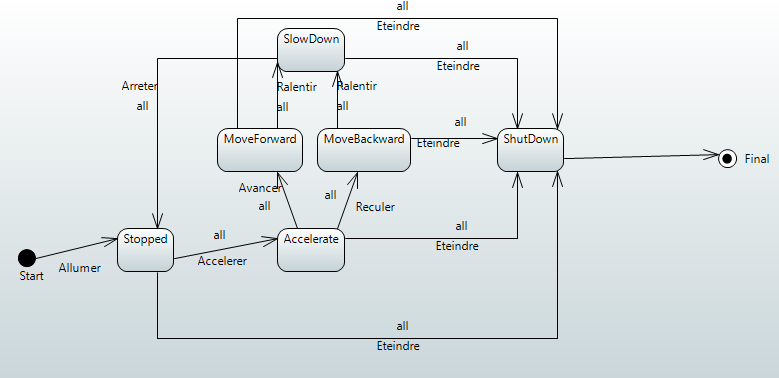
\includegraphics[scale=0.6]{Images/diagrammeV1.png}
				\captionof{figure}{Premier diagramme d'état transition généré}
	\end{center}
    
    \subsubsection{Écriture du code}
    En se basant sur ce résultat de diagramme, nous avons créé à la main un fichier de code qui représenterait notre objectif de génération automatique. A ce niveau, ayant avancé dans nos recherches de framework, nous avions une vague idée du type de framework que nous allions utiliser sans pour autant en avoir un de défini précisément. C'est pourquoi notre objectif de génération avait une structure précise mais pas définitive. 
    Dans ce fichier, nous avons défini une classe pour chaque état, puis une en plus qui correspondait à la classe Application dans laquelle se trouverait le main. 
    Dans les classes des états, nous avons défini que le framework que nous allions employer aurait des méthodes prédéfinies, et que les classes surchargeraient chacune de ces méthodes. 
    
	\begin{lstlisting}[caption={Exemple de classe à générer en utilisant le premier diagramme.},basicstyle=\small]
 // Specific class and methods description for the node <Stopped>
public class Stopped extends Node {
  @Override
  public void onEventStart(){
    //TODO : Complete with the code to execute when an event is called on this node
  }
  @Override
  public void onEventDestination(){
    //TODO : Complete with the code to execute when an event leads to this node
  }
  @Override
  public void onEntering(){
    //TODO : Complete with the code to execute when you enter in this node
  }
  @Override 
  public void onLeaving(){
    //TODO : Complete with the code to execute when you leave this node
  }

	\end{lstlisting}
	
	Pour la classe Application, nous partions du principe que le framework utilisé s'appliquerait sous forme de graphe. En effet, chaque classe serait un noeud du graphe, et chaque transition, appelée ici switch, serait une transition ajoutée à ce graphe. Avec cette méthode, le graphe que nous aurions généré en Java reprendrait quasi-exactement la structure de notre diagramme de départ.
	
	\begin{lstlisting}[caption={Classe application à générer.},basicstyle=\small]

public class Application{
    public static void main(String[] args){
    // Graph initialization
    Graph graph = new Graph();
    
    // Nodes initionazation and adding to the graph
    Stopped stopped = new Stopped();
    graph.addNode(stopped);
    ...
    
    // Set starting nodes of the graph
    graph.setStartingNode(Stopped);
    
    // Set ending nodes of the graph
    graph.setEndingNode(ShutDown);
    
    //Set the transitions
    graph.addSwitch(Stopped, Accelerate, "Accelerer");
    graph.addSwitch(Accelerate, MoveForward, "Avancer");
    ...

    // After graph initialization, run the graph execution
    graph.run();
}
	\end{lstlisting}

    
    \subsubsection{Programmation ATL}
    C'est la partie programmation en ATL qui a posé le plus de difficultés, au moins au début de l'étape. En effet, le tutoriel que nous avions effectué en suivant les conseils de Mohammed Tebib avait permis de relativement bien comprendre le principe général d'ATL, mais nous n'avions alors pas encore généré de code, et nous avions beaucoup de difficultés à visualiser comment nous allions faire. 
    A ce moment là, c'est Mohammed Tebib qui nous a complètement débloqué en nous envoyant le travail que lui avait déjà effectué en appliquant un design pattern State. Nous avons ensuite pu nous baser sur son travail pour comprendre comment itérer sur chaque composant du diagramme et générer chaque partie du code. 
    Contrairement au processus vu dans le tutoriel, pour produire du code nous ne prenions pas deux métamodèles (un source et un cible) et un modèle source afin de générer de modèle cible. En effet, dans notre cas, aucune règle ATL n'était définie. Nous prenions simplement un metamodele et modèle source (le diagramme UML), et nous produisions alors un fichier .java, que nous complétions en retournant des String dans nos helpers. 
    \newline
    Afin de savoir sur quoi itérer, il nous fallait visualiser correctement la structure du diagramme non pas sous la forme graphique mais plutôt sous la forme structurelle.
    
	\begin{center}
			\captionsetup{type=figure}
			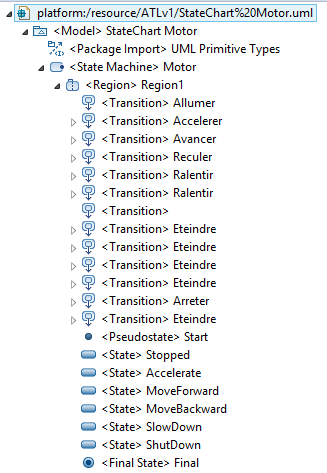
\includegraphics[scale=0.7]{Images/structureV1.png}
			\captionof{figure}{Structure du premier diagramme d'état transition généré}
	\end{center}
	
	En consultant ceci, nous savions donc que pour générer chaque classe correspondante à un état il faudrait entrer dans le state machine, puis dans la région, et récupérer la liste des états. Il faudrait ensuite itérer dessus et créer une classe à chaque fois.
	
	\begin{lstlisting}[caption={Méthode appelant la génération de code pour chaque State Machine du modèle},basicstyle=\small]
helper context MM!Model def : GenerateJavaCode() : String = 
  let  stateMachines : MM!StateMachine = MM!StateMachine.allInstances() in
   '/* \n'
   + ' * Automatically generated Java code with ATL \n'
   + ' */ \n'
   + stateMachines->iterate(it; Class_Code: String = ''|Class_Code 
   + it.getRegion(it))
  ;
  	\end{lstlisting}

      
  \begin{lstlisting}[caption={Méthode appelant la génération de code pour chaque Region du State Machine.},basicstyle=\small]

helper context MM!StateMachine def : getRegion(x:MM!StateMachine) :String=
 let regions : MM!Region = x.region->select(a|a.oclIsTypeOf(MM!Region)) in 
  	 regions->iterate(it; result: String = ''|result 
        + it.generateCode(it))
      ;
	\end{lstlisting}
	
  \begin{lstlisting}[caption={Méthode appelant la génération de code pour chaque State (état) de la région.},basicstyle=\small]

helper context MM!Region def : generateCode(x:MM!Region) : String = 
 let states : MM!State = x.subvertex->select(a|a.oclIsTypeOf(MM!State)) in
		' ' 
		+ x.generateClasses(states)
        ;
	\end{lstlisting}
	
  \begin{lstlisting}[caption={Méthode générant le code de chaque classe correspondante à un état du diagramme.},basicstyle=\small]

helper context MM!Region def : generateClasses(x:MM!State) :  String = 
	x->iterate(it; result:String =''| result
		+ 
        '// Specific class and methods description for the node <' + it.name+'>
    	public class ' + it.name + ' extends Node {
    	
    	  @Override
    	  public void onEventStart(){
    	    //TODO : Complete with the code to execute when an event is called
    	    //on this node
    	  }
    	  ...
    	}\n\n'		
    );

    \end{lstlisting}
    
    Ce processus ayant été assimilé, la suite a été beaucoup plus naturelle car nous avions bien mieux compris comment manier ATL. 
    L'étape suivante de la génération de code était la génération de la classe Application qui contiendrait le main, dans laquelle nous créerions nous graphe (structure du framework), et dans laquelle nous ajouterions à ce graphe les classes en tant que noeud, les états initiaux et finaux et les transitions.
    La création du graphe en lui-même se faisait en texte dur, sans avoir besoin d'utiliser les attributs du diagramme d'état-transition. 
    L'initialisation des classes et l'ajout de celles-ci en tant que noeud s'est faite en itérant à nouveau sur les nom des états et en créant une String utilisant ce nom à chaque fois. 
    
      \begin{lstlisting}[caption={Création de l'arbre et des classes et ajout des noeuds dans l'arbre.},basicstyle=\small]

helper context MM!Region def :generateApplicationClass(x:MM!State):String=
	'public class Application{
        public static void main(String[] args){
            // Graph initialization
            Graph graph = new Graph();
        
            // Nodes initionazation and adding to the graph\n'
        	    + x->iterate(it; result:String =''| result
        		+ it.name
        		+ ' '
        		+ it.name.toLowerCase()
        		+ ' = new '
        		+ it.name
        		+'();\n'
        		+ 'graph.addNode('
        		+ it.name.toLowerCase()
        		+ ');\n\n'
	            );

    \end{lstlisting}
    
L'étape suivant était la génération des noeuds d'entrée et de sortie correspondant aux états initiaux et terminaux du graphe. Pour cette partie, des conditionnelles ont dû être mises en place en ATL, ce que nous n'avions encore jamais fait, mais qui était tout de même très simple car très similaire à tous les autres langages de programmation.
Dans notre diagramme, l'état d'entrée était "Stopped", car il était celui sur lequel pointait le InitialState. Il fallait donc en ATL récupérer l'InitialState, récupérer la transition dont il était la source, puis récupérer la cible de cette transition. 

  \begin{lstlisting}[caption={Création de l'état initial du graphe correspondant à l'état entrant du diagramme.},basicstyle=\small]

helper context MM!Region def : generateInitial(x:MM!Pseudostate, trans:MM!Transition, states:MM!State) : String =
	'// Set starting nodes of the graph\n'
	+ x->iterate(it; result: String = ''|result
	    //recherche parmis les transitions de celle dont la source est l'InitialState (ici, pseudoState)
		+trans->iterate(its; results: String = ''|results
			+''
			+ if(its.source=it) then 
			    //Quand elle a ete trouvee, on recupere sa cible et definit que celle-ci sera l'etat initial du graphe en Java
				states->select(a|a=its.target)->iterate(itp; resultp: String = ''|resultp
					+'graph.setStartingNode('
					+ itp.name
					+ ');\n\n'
					)
			else '' 
			endif
		)
	);

    \end{lstlisting}
    
Pour ce qui est de l'état final, le processus est identique, sauf que l'on recherche la source de la transition dont la cible et le FinalState du diagramme.

Enfin, il fallait ajouter au graphe Java toutes les transitions. Pour cela, il fallait simplement récupérer toutes les transitions qui n'avaient pas pour source un InitialState ou pour cible un FinalState (car déjà traitée juste avant), et créer une ligne de code java pour chaque. 

  \begin{lstlisting}[caption={Création des transitions dans le grpahe Java en utilisant les transitions du diagramme},basicstyle=\small]

helper context MM!Region def :  generateTransitions(x:MM!Transition) : String = 
	'//Set the transitions\n'
	+ x->iterate(it; result: String = ''|result
		+ ''
		+ if(it.toString()<>'OclUndefined') then 
			if(it.source.oclIsTypeOf(MM!Pseudostate)=false) then
				if(it.target.oclIsTypeOf(MM!FinalState)=false) then
    				'graph.addSwitch('
    				+it.source.name +', '
					+it.target.name +', "'
					+it.name +'");\n'
				else '' 
				endif
			else '' 
			endif
		else '' 
		endif
	);

    \end{lstlisting}

Ce code assemblé nous a permis d'obtenir exactement le code souhaité dans notre objectif de génération en utilisant les différents attributs du diagramme.     
Tout ceci étant mis en place, nous avions un programme ATL qui prenait en entrée un diagramme d'état-transition de la même structure que le notre, et qui produisait du code Java correspondant, en suivant une structure utilisant un framework encore non défini précisément, mais dont le principe général était celui employé. 

\subsection{Génération avec un framework précis}
    Au moment où nous sommes parvenus à générer tout le code du diagramme précédents, nous avons enfin opté pour un framework précis qui convenait à nos attentes et nos besoins. Comme mentionné précédemment, nous avons donc décidé que le Statechart Framework serait utilisé. Nous avons donc gardé la version précédente en tant que première version, et nous avons recommencé, en nous basant sur le travail précédent, une autre génération de code qui correspondait à la nouvelle structure de diagramme ainsi qu'à la nouvelle structure de code.
    
    \subsubsection{Création du diagramme}
    Le second diagramme que nous avons créé a été réalisé avec beaucoup plus de minutie que le premier, puisque nous avions une structure bien définie à suivre afin de pouvoir faire correspondre efficacement le code au diagramme.
    
    Le diagramme obtenu est le suivant : 
    \begin{center}
			\captionsetup{type=figure}
			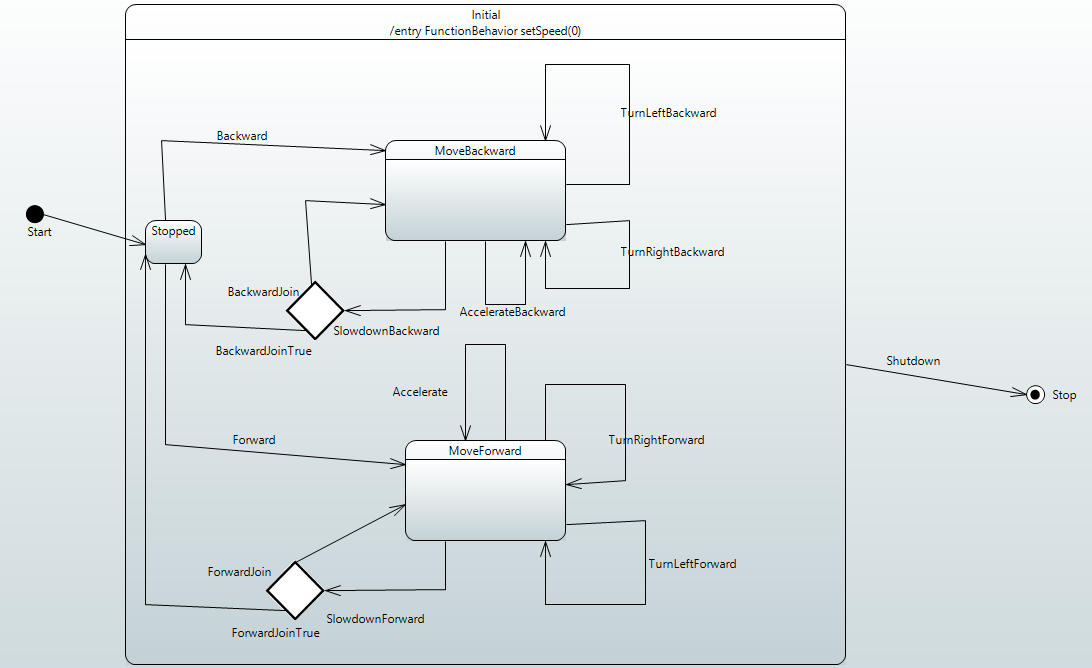
\includegraphics[scale=0.6]{Images/diagrammeV2.PNG}
			\captionof{figure}{Second diagramme d'état transition généré}
	\end{center}
	
	Cependant, après avoir créé le diagramme, nous avons rencontré des difficultés avec Papyrus, car certaines informations ont disparu lorsque nous avons exporté le diagramme afin de l'inclure dans l'ATL. En effet, il devait normalement y avoir sur chaque transition un label, qui correspondrait en code à un nom de fonction à créer. Ceux-ci étant présents à la création du diagramme, ils ont  complètement disparu lorsque le diagramme a été exporté. 
    

    \subsubsection{Écriture du code}
    En se basant sur le diagramme, sur le code de la première version mais surtout sur les indications du framework, nous avons généré un fichier d'objectif de code en suivant chaque étape de création du code fourni par la documentation du framework. Le fichier contient donc pour chaque transition du diagramme une classe correspondante à l'évènement :
 
  \begin{lstlisting}[caption={Création d'une des classes évènement correspondantes aux transitions},basicstyle=\small]

// Event corresponding to "Forward"
public class ForwardEvent extends Event {
  public void ForwardEvent() {
    super("Forward");
  }
}
    \end{lstlisting}
    
    Ensuite, comme demandé dans la documentation du framework, nous avons généré une classe par action à effectuer par le robot : 
  
  \begin{lstlisting}[caption={Création d'une des classes correspondantes aux actions},basicstyle=\small]

// Action corresponding to "increaseSpeed()"
public class IncreaseSpeed extends Action {
  public void execute(Metadata data, Parameter parameter) {
    //TODO: complete this function
  }
}
    \end{lstlisting}
    
    L'étape suivante était la génération des guards, donc des classes qui permettrait de vérifier si des conditions étaient respectées ou non : 
    
  \begin{lstlisting}[caption={Création du seul guard que nous utilisons},basicstyle=\small]

// Guard corresponding to "SpeedEquals(...)"
public class SpeedEquals extends Guard {
  private int value;

  public SpeedEquals(int value) {
   this.value = value;
  }

  public boolean check(Metadata data, Parameter parameter) {
    //TODO: complete this function
  }
}
    \end{lstlisting}
    
    Ensuite, une classe Metadata était nécéssaire pour instancier les variables utilisées dans les fonctions : 
    
      \begin{lstlisting}[caption={Création de la classe metadata},basicstyle=\small]

// Metadata creation
public class MyMetadata extends Metadata {
  //TODO: add variables used in functions
}
    \end{lstlisting}
    
    Enfin, le code se terminait par la classe Application contenant le main, dans laquelle sont instanciées les différentes classes créées, et ajoutées au Statechart (le coeur de notre framework). Sont ensuite créées des transitions, qui relieront les états entre eux, en indiquant l'évènement et la fonction à appeler pour chacune (si ces informations sont nécessaires). Pour terminer, une instance de la classe metadata est créée, et le statechart est "lancé".
    
  \begin{lstlisting}[caption={Création de la classe Application},basicstyle=\small]

// Main Application
public class Application{

  public static void main(String[] args){

    // Statechart initialisation
    Statechart statechart = new Statechart();

    // Main states creation
    PseudoState startState = new PseudoState("Start", statechart, PseudoState.pseudostate_start);
    FinalState stopState = new FinalState("Stop", statechart);
    State initialState = new State("Initial", statechart);

    // Initial states creation
    State stoppedState = new State("Stopped", initialState);
    State moveFowardState = new State("MoveFoward", initialState);
    ...

    // Transitions from state "Start"
    new Transition(startState, stoppedState);

    // Transitions from state "Initial"
    new Transition(initialState, stoppedState, new ShutdownEvent(), new Shutdown());
    ...

    //Run the statechart
    MyMetadata myMetadata = new MyMetadata();
    chart.start(myMetadata);

  }
    \end{lstlisting}
    
    En ayant suivi chaque étape précisée par la documentation du framework, nous sommes donc parvenus à obtenir un fichier d'objectif de génération de code complet qui correspondait à nos attentes.
    
    \subsubsection{Programmation ATL}
    Ayant des informations manquantes sur le diagramme (les labels ayant disparu), nous avons commencé à mettre en place tout ce que nous pouvions en faisant abstraction des difficultés, et en laissant pour l'instant de coté les parties nécessitant les-dites informations. 
    
    Le diagramme ayant changé de structure, il fallait recommencer à visualiser celle-ci afin de connaître la structure des éléments (lesquels sont imbriqués dans lesquels, etc.)
    
	\begin{center}
			\captionsetup{type=figure}
			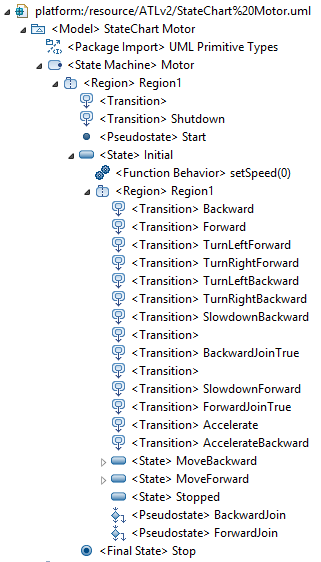
\includegraphics[scale=0.7]{Images/structureV2.png}
			\captionof{figure}{Structure du second diagramme d'état transition généré}
	\end{center}
	
	Nous remarquons que, à la différence du premier diagramme, nous avons un état général qui contient une région dans laquelle sont imbriqués d'autres états et transitions. Bien que ceci ne représente rien de particulièrement complexe à première vue, cela signifiera qu'un plus grand nombre d'itérations sera nécessaire dans notre code ATL pour aller chercher les informations situées plus en profondeur.
    
    En suivant le même cheminement que pour créer l'objectif de génération de code, nous avons commencé par mettre en place les classes évènement correspondantes aux transitions. Ceci a été fait en deux parties car comme nous pouvons le constater dans la structure du diagramme, une des transitions ne se situe pas à la même profondeur que les autres. Pour créer celle-ci, nous avons donc utilisé le même code que pour le premier diagramme, puisque cette partie de la structure était la même. Pour les autres transitions, il a fallu aller chercher l'état puis la région les contenant.
    
    \begin{lstlisting}[caption={Création de la classe évènement de la première transition, la moins profonde},basicstyle=\small]

helper context MM!Region def :generateFirstTrans(x:MM!Transition):String = 
	x->iterate(it; result: String = ''|result
		+ if(it.name.toString()<>'OclUndefined') then 
            '\n// Event corresponding to "' + it.name + '"
            	 public class '+it.name+'Event extends Event {
            			public '+it.name+'Event() {
            	 			super("'+it.name+'");
            	 	    }
            	 }'
		else '' 
		endif
	);
    \end{lstlisting}
    
    \begin{lstlisting}[caption={Création des autres classes d'évenements},basicstyle=\small]

//Recuperation de la region dans l'etat
helper context MM!Region def :  generateClasses(x:MM!State) : String = 
	let region : MM!Region=x.region->select(a|a.oclIsTypeOf(MM!Region)) in 
		region->iterate(it; result: String = ''|result
			+x.generateCodeFromRegion(it)
	);

//Recuperation des transitions et generation de celles-ci
helper context MM!State def : generateCodeFromRegion(x:MM!Region):String = 
	let transitions : MM!Transition = x.transition->select(a|a.oclIsTypeOf(MM!Transition)) in
	let pseudoStates : MM!Pseudostate = x.subvertex->select(a|a.oclIsTypeOf(MM!Pseudostate)) in
			x.generateTransitions(transitions,pseudoStates)
	;

//Generation du code des transitions, en ne prenant pas les transitions ayant pour source les pseudo-etats
helper context MM!Region def : generateTransitions(x:MM!Transition, y:MM!Pseudostate) : String = 
		x->iterate(it; result: String = ''|result
		+if(it.name.toString()<>'OclUndefined') then 
			if(it.source.oclIsTypeOf(MM!Pseudostate)=false) then
                '\n// Event corresponding to "' + it.name + '"
                	 public class '+it.name+'Event extends Event {
                			public '+it.name+'Event() {
                	 			super("'+it.name+'");
                	 	}
                	}'
			else '' 
			endif
		else ''
		endif
		);
    \end{lstlisting}
    
    L'étape suivante était normalement la génération des classes d'actions utilisant les labels des transitions. Ceux-ci ayant disparu et commençant à manquer de temps, nous avons laissé cette partie de coté. En effet, cette partie est à ce niveau générée en ayant mis le code java complet en dur dans la génération, et elle ne dépend donc pas du tout du diagramme en entrée.\\
    Le même problème s'est posé pour la génération du guard, puisqu'ici aussi, la variable du nom de la méthode que nous aurions du exploiter était stockée dans les labels ayant disparu.
    
    Ensuite, il fallait générer la classe metadata. Celle-ci ne dépendant en rien des attributs du diagramme, nous avons pu la générer directement en dur en ATL : 
    \begin{lstlisting}[caption={Génération de la classe metadata},basicstyle=\small]

helper context MM!Region def : generateMetadata() : String = 
    '// Metadata creation
    public class MyMetadata extends Metadata {
      //TODO: add variables used in functions
    }'
;
    \end{lstlisting}
    
    La dernière classe à générer était la classe Application. Il a donc fallu la créer mais surtout la remplir. Pour cela, nous avons commencé par implémenter le début de la classe qui ne dépend pas du graphe et qui peut donc être généré directement. Ensuite, il fallait instancier les trois états principaux : l'initial, le final, et l'état général contenant la région et toutes les autres informations. 
    Pour cela, nous pouvions reprendre le code utilisé dans la première version. En effet, il nous suffisait de récupérer le pseudoState, le finalState et le state de la bonne profondeur et de générer une ligne de code pour chacun.
    
        \begin{lstlisting}[caption={Extrait de la méthode récupérant les différents états et appelant la génération sur chacun},basicstyle=\small]
        
helper context MM!Region def : generateCode(x:MM!Region) : String = 
    //Recuperation des etats principaux
	let stateRegion : MM!State = x.subvertex->select(a|a.oclIsTypeOf(MM!State)) in
	//Recuperation des etats initiaux
	let initials : MM!Pseudostate = x.subvertex->select(a|a.oclIsTypeOf(MM!Pseudostate)) in
	//Recuperation des etats finaux
	let finals : MM!FinalState = x.subvertex->select(a|a.oclIsTypeOf(MM!FinalState)) in
		' ' 
		+ x.generateInitialState(initials)
		+ x.generateFinalState(finals)
		+ x.generateState(stateRegion)
	;
	    \end{lstlisting}

        \begin{lstlisting}[caption={Méthodes de génération des lignes de code pour chaque type d'état},basicstyle=\small]
        
helper context MM!Region def : generateInitial(x:MM!Pseudostate):String = 
	x->iterate(it; result: String = ''|result
		+'	PseudoState '+it.name.toLowerCase()+'State = new PseudoState("'+it.name+'", statechart, PseudoState.pseudostate_start);\n'
	);

helper context MM!Region def :  generateFinal(x:MM!FinalState) : String = 
	x->iterate(it; result: String = ''|result
		+'	FinalState '+it.name.toLowerCase()+'State = new FinalState("'+it.name+'", statechart);\n'
	);

helper context MM!Region def :  generateState(x:MM!State) : String = 
	x->iterate(it; result: String = ''|result
		+'	State '+it.name.toLowerCase()+'State = new State("'+it.name+'", statechart);\n'
	);
    \end{lstlisting}
    
    Ensuite, il nous fallait générer les états contenus dans l'état principal. Pour cette partie, nous prenons comme pré-requis qu'il n'y ait qu'un seul état principal, un seul état final, et un seul état initial, et nous utiliserons les noms que nous avons décidé en instanciant ces derniers. En effet, la génération des sous-états prenait en paramètre l'état principal contenant tous les sous-états. Nous devions donc définir à l'état principal un nom précis, et l'utiliser pour le passer en paramètre afin de créer correctement les lignes de codes pour cette partie. Afin de mettre en place cette étape, nous devions descendre dans la profondeur afin de récupérer les états imbriqués dans l'état principal.
    
    \begin{lstlisting}[caption={Méthodes de génération des lignes de code pour chaque sous-état, en fonction de son type},basicstyle=\small]

//Recuperation de la region dans l'etat principal        
helper context MM!Region def :  generateAllStates(x:MM!State) : String = 
	let region : MM!Region=x.region->select(a|a.oclIsTypeOf(MM!Region)) in 
		region->iterate(it; result: String = ''|result
			+x.generateStatesCode(it)
	);

//Recuperation des sous-etats et appel des methodes de generation 
helper context MM!State def :  generateStatesCode(x:MM!Region) : String = 
	let states:MM!State=x.subvertex->select(a|a.oclIsTypeOf(MM!State)) in
	let pseudoStates : MM!Pseudostate = x.subvertex->select(a|a.oclIsTypeOf(MM!Pseudostate)) in
		'\n    // Initial states creation		\n'
		+ x.generateNormalStates(states)
		+ x.generatePseudoStates(pseudoStates)	
	;

//Generation du code pour un etat normal
helper context MM!Region def : generateNormalStates(x:MM!State) : String = 
		x->iterate(it; result: String = ''|result
		+'    State '+it.name.toLowerCase()+'State = new State("'+it.name+'", initialState);\n'
		);

//Generation du code pour un pseudo etat
helper context MM!Region def : generatePseudoStates(x:MM!State) : String = 
		x->iterate(it; result: String = ''|result
		+'    PseudoState '+it.name.toLowerCase()+'PseudoState = new State("'+it.name+'", initialState);\n'
		);
    \end{lstlisting}
    
    Lors de l'avant dernière étape, nous avons rencontré le même problème que précédemment, car nous avions besoin pour générer les transitions des noms des classes d'actions. Ne possédant pas ces informations, nous avons laissé cette partie de coté et implémenté le code en écrivant directement dans l'ATL le code à générer, sans mettre en place de dépendance avec le diagramme.
    
    Enfin, la dernière étape ne demandait quant à elle pas de dépendance avec le code, puisqu'il s'agissait simplement d'instancier la classe metadata et de "lancer" le statechart. Ceci peut donc se faire directement dans l'ATL, sans qu'il ne soit vraiment nécessaire de le faire dans une méthode à part.

C'est à ce point que s'est terminé notre projet, en ayant obtenu un code complet pour la première version ainsi qu'un code à compléter pour la seconde version.

        \subsubsection{Fonctionnalités inexploitées du framework}
        De part le temps qui nous était imparti, nous avons créé un diagramme de state machine permettant de mettre en place le déplacement du robot de manière élémentaire. Certaines fonctionnalités du framework n'ont ainsi pas été exploitées bien que pouvant se montrer utiles dans les travaux à venir. (Les images utilisées à titre d'exemple dans cette partie proviennent du git du framework.)
        
        \paragraph{Time-triggerd : }
        Une notion essentielle dans tout programme d'exécution en temps réel est la gestion de temps. Cette dernière a été implémentée au sein du framework par la classe TimeoutEvent. Un évènement classique doit être hérité de la classe Event, afin d'en créer une version spécifique, et sera responsable de la transition d'un état à un autre lorsque l'évènement en question sera perçu part le Statechart (le graphe principal gérant l'exécution) . Pour le TimeoutEvent, il n'est pas nécessaire d'hériter de la classe, en créer une instance avec le temps souhaité suffira, ces instances n'auront pas besoin d'être stockées, l'évènement engendrant de lui même la transition souhaitée lorsque le Statechart le lui demande.
        \bigskip
        
        D'un point de vue graphique le TimeoutEvent peut être représenté de la façon suivante :
        
        \begin{center}
			\captionsetup{type=figure}
			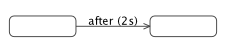
\includegraphics[scale=1]{Images/time_triggered_transition.png}
			\captionof{figure}{Représentation d'un évènement de type Time-triggered}
	    \end{center}
	    
	   Et il peut être instancié de la façon suivante :
        
         \begin{lstlisting}[basicstyle=\small]

// Definition de l'etat 'a' et 'b'
State state_a = new State("a", statechart);
State state_b = new State("b", statechart);

// Transition effectuees automatiquement de 'a' vers 'b' apres 1000 ms d'attente 
new Transition(state_a, state_b, new TimeoutEvent(1000));
        \end{lstlisting}
        
        
        \paragraph{Transitions segmentées : }
        La notion de transition segmentée permet de découper la transition d'un état à un autre en plusieurs étapes, chaque étape permettant d'exécuter une fonction différente, plutôt que de n'avoir qu'une transition directe de l'état 'a' à l'état 'b' exécutant une fonction plus conséquente regroupant toutes les exécutions. Cette notion est utile dans le cas ou l'on souhaite éviter la multiplication de fonctions imposantes correspondantes à des cas spécifiques, ce qui est notre cas, étant donné que chaque fonction engendrera la création d'une classe et donc nécessitera plus d'organisation. L'idée ici est donc de pouvoir créer des fonctions plus élémentaires qui associées ensembles et mises bout à bout recréent le comportement général.
        
        \bigskip
        
        Dans l'exemple ci-dessous, lorsque l'évènement S1 est perçu par l'état de gauche, si la variable x vaut 1, alors on exécutera la fonction a1, puis la fonction a2, et sinon la transition se fera sans exécution.
        
         \begin{center}
			\captionsetup{type=figure}
			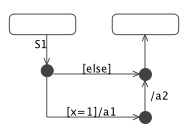
\includegraphics[scale=1]{Images/segmented_transition.png}
			\captionof{figure}{Représentation d'une transition segmentée}
	    \end{center}
        
        Cet exemple pourrait être implémenté de cette façon :
        
        \begin{lstlisting}[basicstyle=\small]
//...

// Definition de l'etat 'a' et 'b'
State state_a = new State("a", statechart);
State state_b = new State("b", statechart);

// Definition des trois etats qui vont segmenter notre transition
PseudoState state_j1 = new PseudoState("j1", statechart, PseudoState.pseudostate_junction);
PseudoState state_j2 = new PseudoState("j2", statechart, PseudoState.pseudostate_junction);
PseudoState state_j3 = new PseudoState("j3", statechart, PseudoState.pseudostate_junction);

// Effectuer une transition de 'a' vers 'j1' lorsque l'evenement 'S1' est percu
new Transition(state_a, state_j1, new S1());

// Effectuer une transition de 'j1' vers 'j2' si XEquals(1) renvoie 'true', puis executer A1()
new Transition(state_j1, state_j2, new XEquals(1), new A1());

// Effectuer une transition de 'j1' vers 'j3' si aucune autre transition precedente n'a ete execute
new Transition(state_j1, state_j3, new S1());

// Effectuer une transition de 'j2' a 'j3' et executer A2()
new Transition(state_j2, state_j3, new A2());

// Effectuer une transition de 'j3' a 'b'
new Transition(state_j3, state_b);
        \end{lstlisting}
        
        
        \paragraph{Hierarchical states : }
        De manière à décrire un état complexe, un état peut contenir plusieurs états qui vont spécifier le fonctionnement global de l'état principal. L'état principal peut alors posséder un état de départ et plusieurs états de fin. De ce fait, si un évènement conduit l'exécution à l'état principal, l'exécution continuera son chemin à partir de l'état de départ de l'état principal. De la même manière si une transition sans évènement part de l'état principal, il faudra atteindre un état de sorti de l'état principal pour pouvoir effectuer cette transition. 
        
        Il est bon de noter que les états contenus dans l'état principal ne sont pas obligés de passer par les états d'entrée et de sortie pour interagir avec l'extérieur de l'état principal, des transitions entrantes ou sortantes peuvent directement connecter les états intérieur à l'extérieur.
        
         \begin{center}
			\captionsetup{type=figure}
			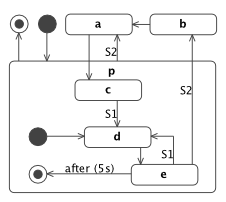
\includegraphics[scale=1]{Images/hierarchical_states.png}
			\captionof{figure}{Représentation d'une hiérarchie d'états}
	    \end{center}
        
        Il est possible de voir sur l'exemple ci-dessus le cas particulier de l'évènement S2. Cet évènement est en sorti de l'état principal ainsi que de l'état 'e'. De fait, si l'état courant est l'état 'e', alors sa transition sera suivie en priorité. Pour n'importe quel autre état contenu dans l'état principal, la transition de l'état principal, pour l'évènement S2, sera suivie si l'évènement est relevé.
        
        On peut également observer ce qui pourrait être considéré comme un système de mise en veille, l'état 'e' reste l'état courant pendant un maximum de 5 secondes. Si un évènement est perçu avant la fin de ce temps, l'exécution continue et le compte à rebours se relance, sinon la transition de 'e' vers l'état de fin de l'état principal se fait, enchaînée avec la transition de l'état principal vers l'état de fin du Statechart.
        \bigskip
        
        Voici une implémentation pouvant engendrer ce diagramme :
        
        \begin{lstlisting}[basicstyle=\small]
// Creation du statechart et attribution de son point de debut et de fin
Statechart statechart = new Statechart();
PseudoState state_start = new PseudoState("start", statechart, PseudoState.pseudostate_start);
FinalState state_final = new FinalState("final", statechart);

// Creation de l'etat 'a' et 'b'
State state_a = new State("a", statechart);
State state_b = new State("b", statechart);

//Creation de l'etat principal et de tous les etats le constituant
HierarchicalState  state_p = new HierarchicalState ("principal", statechart);
PseudoState p_start = new PseudoState("start", state_p, PseudoState.pseudostate_start);
FinalState p_final = new FinalState("final", state_p);
State state_a = new State("c", state_p);
State state_b = new State("d", state_p);
State state_b = new State("e", state_p);

//Definition de toutes les transitions
new Transition(state_start, state_p);

new Transition(p_start, state_d);

new Transition(state_a, state_c);

new Transition(state_b, state_a);

new Transition(state_c, state_d, new S1());

new Transition(state_d, state_e);

new Transition(state_e, state_d, new S1());
new Transition(state_e, state_b, new S2());
new Transition(state_e, p_final, new TimeoutEvent(5000));

new Transition(state_p, state_a, new S2());
new Transition(state_p, state_final);

        \end{lstlisting}
        
        \paragraph{History states : }
        Un autre élément important pouvant être associé avec le système de hiérarchie d'états est le "history state". Le principe du history state est de se souvenir de quels étaient les états actifs au sein d'un état principal. Il existe deux types d'history state, le "shallow history", noté "H", permet de retenir quel était le dernier sous-état direct en activité, alors que le "deep history", noté "H*", retiendra l'ensemble des états qui constituent la hiérarchie menant de l'état principal au dernier sous-état actif.

        \begin{center}
			\captionsetup{type=figure}
			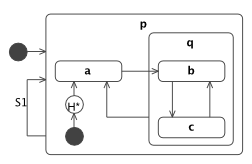
\includegraphics[scale=1]{Images/History_state.png}
			\captionof{figure}{Exemple d'utilisation d'un history state}
	    \end{center}

        Dans cet exemple on peut observer la présence d'un "deep history" à l'entrée de l'état 'p'. De fait, si l'évènement S1 est relevé pendant l'exécution, le cour de l'exécution va s'arrêter en sortant de 'p', puis va recommencer à l'état de départ de 'p'. L'history state contenant le dernier état actif, l'exécution reprendra à l'état en question comme si elle n'avait pas été interrompue. Si, par contre, c'est la première fois que l'on passe par 'H*', ne contenant pas d'historique, il aurait simplement déclenché la transition vers l'état 'a'.
        
        On peut observer la différence entre 'H' et 'H*' avec cet exemple. Partons du principe que l'évènement S1 est appelé alors que l'état courant est 'b'. Si l'history state était un shallow state, soit 'H', l'information qu'il aurait stocké aurait été que le dernier sous-état direct actif était 'q' car il contient 'b' qui était le dernier actif. Avec le deep history, soit 'H*', l'information stockée aurait été un arbre indiquant qu'au sein de 'p', 'q' était actif et qu'au seins de 'q', 'b' était actif. Dans le deuxième cas, l'exécution reprendra donc à 'b' alors que dans le premier elle reprendra au point de départ de 'q' (bien qu'ici il n'en ait pas).
        \bigskip
        
        Il est possible de créer des history states de la façon suivante :
        
        \begin{lstlisting}[basicstyle=\small]
        //...

PseudoState sh = new PseudoState("H", statechart, PseudoState.pseudostate_history);
PseudoState dh = new PseudoState("H*", statechart, PseudoState.pseudostate_deep_history);

        \end{lstlisting}
        
        
        \paragraph{Les régions : }
        Le principe de région sert à découper un état principal en plusieurs régions, chaque région aura alors son propre point de début et de fin, les régions s'exécuteront parallèlement. Toute transition entrante sur l'état principal entraînera l'exécution parallèle de toutes les régions, cela vaut même si la transition entrante n'arrive pas sur l'état principal mais directement sur un état contenu dans une région. Pour ce qui est de la terminaison, si toutes les régions atteignent leur état de fin, alors l'état principal déclenche sa transition de sortie, par contre si l'une des régions sort de l'état principal sans passer par son état de fin, alors toutes les régions sont interrompues dans leur exécution, tous les sous états devant continuellement s'exécuter en parallèle.
        
         \begin{center}
			\captionsetup{type=figure}
			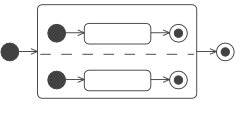
\includegraphics[scale=1]{Images/region_state.png}
			\captionof{figure}{Représentation d'un état principal possédant deux régions}
	    \end{center}
	    
	    Bien que schématique, l'exemple ci-dessus pourrait être implémenter de la façon suivante :
	    
	    \begin{lstlisting}[basicstyle=\small]
Statechart statechart = new Statechart();
PseudoState state_start = new PseudoState("start", statechart, PseudoState.pseudostate_start);
FinalState state_final = new FinalState("final", statechart);

// Creation de la zone de concurrence
ConcurrentState state_c = new ConcurrentState("c", statechart);

// Region 1 de la zone de concurrence
HierarchicalState state_c_r1 = new HierarchicalState("c_r1", state_c);

// Contenu de la region 1
PseudoState c_r1_start = new PseudoState("c_r1_start", state_c_r1, PseudoState.pseudostate_start);
FinalState c_r1_final = new FinalState("c_r1_final", state_c_r1);
State state_a = new State("a", state_c_r1);

// Region 2 de la zone de concurrence
HierarchicalState state_c_r2 = new HierarchicalState("c_r2", state_c);

// Contenu de la region 2
PseudoState c_r2_start = new PseudoState("c_r2_start", state_c_r2, PseudoState.pseudostate_start);
FinalState c_r2_final = new FinalState("c_r2_final", state_c_r2);
State state_b = new State("b", state_c_r2);


// Definition des transitions
new Transition(state_start, state_c);

new Transition(c_r1_start, state_a);

new Transition(c_r2_start, state_b);

new Transition(state_a, c_r1_final);

new Transition(state_b, c_r2_final);

new Transition(state_c, state_final);

        \end{lstlisting}


\section{Conclusion}
Après une prise en main du projet qui a duré plus longtemps que prévu, nous avons enfin su exactement vers où nous diriger et avons alors pu nous lancer dans l'élaboration des diagrammes et du code ATL. Malgré plusieurs difficultés telles que des soucis de modélisation avec les différents logiciels, le fait que nous n'avions jamais manipulé ATL, que le principe de transformation nous était totalement inconnu au début du projet, ou encore le contexte exceptionnel de confinement qui a énormément perturbé l'organisation, nous sommes parvenus à maintenir l'avancement du projet ainsi que la communication entre tous les acteurs. Les premières productions de code grâce à ATL après avoir pris comme exemple le code de Mohammed Tebib ont été un grand soulagement pour nous, car nous étions auparavant en difficulté sur ce point. La suite s'est alors très bien enchaînée, et nous avons pu progresser efficacement. 
\newline
\newline
Par manque de temps et à cause du contexte spécial principalement, nous avons dû nous arrêter avant d'avoir pu générer la totalité de notre objectif. Cependant, nous pensons que cette partie peut-être complétée relativement simplement à partir du moment où les soucis rencontrés avec les logiciels de modélisation UML sont contournés, ce que nous ne sommes pas parvenus à faire.

De plus, une mise à jour du framework serait à mettre en place. En effet, le framework est adapté à l'UML 1.5 pour les StateMachine, hors nous sommes aujourd'hui à l'UML 2.4.
\newline
\newline
Enfin, il est important de ne pas oublier que l'objectif principal du TER était de découvrir le milieu de la recherche. Nous avons en effet, dans le cadre de ce projet, découvert un travail conséquent ayant été enrichi au cours des années par les différentes équipes y ayant participé. A ce titre, nous avons pu découvrir les conséquences que pouvaient avoir des travaux parallèles ayant été construits sans réels liens les uns avec les autres. Le manque de documentation, ou le fait que cette dernière ne soit plus à jour en vu des nouvelles technologies, a entraîné par exemple l'impossibilité de comprendre ou d'utiliser certains des fichiers fournis. L'avancée dans ce projet s'en est trouvée fortement ralentie et ce travail aurait certainement pu ne jamais aboutir si nous n'avions pas eu les conseils directs de M.André et de Mohammed Tebib, que nous tenons à remercier pour leur aide et leurs conseils tout au long du projet.

Nous pouvons tirer de cette expérience une nouvelle preuve de l'importance de l'organisation et de la documentation en voie au partage et à la réutilisation du travail effectué, concept au coeur même de la filière du master ALMA.


\newpage
\section{Annexe}
\subsection{Faire fonctionner les fichiers ATL}
Afin d'exécuter un fichier ATL, il est nécessaire de le faire avec une configuration précise. Dans notre cas, la voici : 
	\begin{center}
			\captionsetup{type=figure}
			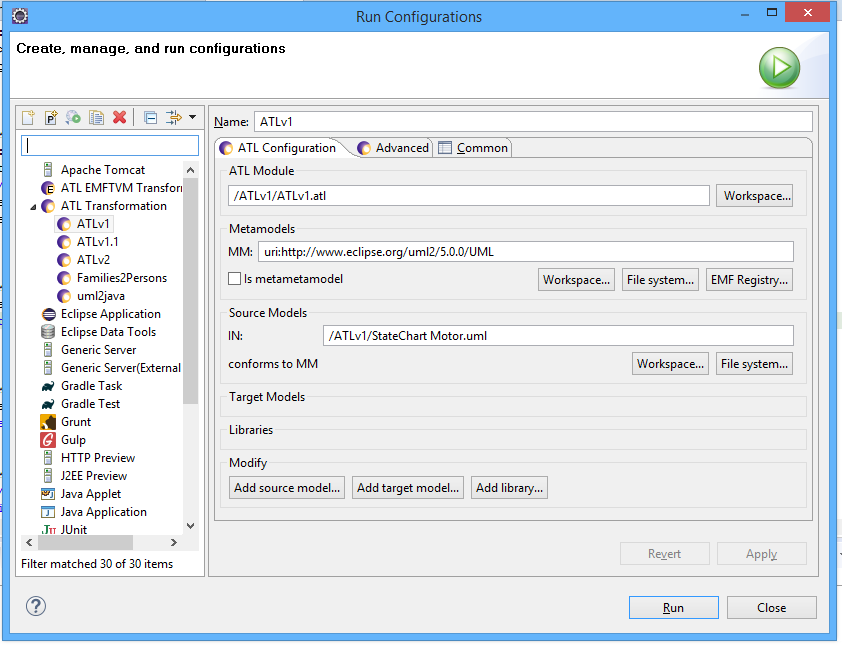
\includegraphics[scale=0.7]{Images/configurationATL.png}
			\captionof{figure}{Configuration pour notre fichier ATL}
	\end{center}
	
	Comme nous pouvons le constater, il est nécessaire de renseigner dans le premier champ le chemin du fichier ATL à exécuter. Ensuite, pour le métamodèle, il faut renseigner le lien vers le métamodèle UML. Puis, dans le modèle source, il faut renseigner le fichier .uml du diagramme que l'on souhaite transformer.
	
	Enfin, afin que le code produit soit un fichier java placé au bon endroit, il est nécessaire de préciser dans la première ligne du fichier ATL que l'on souhaite exécuter où il faudra aller écrire, et quelle est la première méthode à appeler (ici, GenerateJavaCode()).
	    \begin{lstlisting}[basicstyle=\small]
query Script = MM!Model->allInstances()->asSequence().first().GenerateJavaCode().writeTo('/ATLv2/JavaTargetModels/main.java');
        \end{lstlisting}

\end{document}
